\documentclass[tikz,border=8pt]{standalone}
\usepackage{amsmath}
\usepackage{sfmath}
\usetikzlibrary{arrows.meta,positioning,calc,fit,backgrounds}

\definecolor{ink}{RGB}{28,35,45}
\definecolor{muted}{RGB}{84,96,112}
\definecolor{paper}{RGB}{248,250,252}
\definecolor{panel}{RGB}{255,255,255}
\definecolor{line}{RGB}{201,210,224}
\definecolor{mha}{RGB}{40,122,184}
\definecolor{mhafill}{RGB}{232,244,255}
\definecolor{lsso}{RGB}{113,84,179}
\definecolor{lssofill}{RGB}{244,240,255}
\definecolor{green}{RGB}{47,143,85}
\definecolor{greenfill}{RGB}{238,250,242}
\definecolor{amber}{RGB}{210,131,31}
\definecolor{amberfill}{RGB}{255,247,230}

\tikzset{
  font=\sffamily,
  block/.style={draw=ink, very thick, rounded corners=5pt, fill=panel,
    align=center, minimum height=8mm, inner xsep=5mm, inner ysep=2.5mm},
  smallblock/.style={draw=ink, thick, rounded corners=4pt, fill=panel,
    align=center, minimum height=7mm, inner xsep=3mm, inner ysep=2mm},
  mhaBlock/.style={block, draw=mha, fill=mhafill},
  lssoBlock/.style={block, draw=lsso, fill=lssofill},
  stateBlock/.style={block, draw=green, fill=greenfill},
  noteBlock/.style={draw=line, thick, rounded corners=5pt, fill=panel,
    align=left, inner xsep=4mm, inner ysep=3mm},
  panelBox/.style={draw=line, very thick, rounded corners=8pt, fill=panel},
  arrow/.style={-{Latex[length=3mm]}, very thick, draw=ink},
  mhaArrow/.style={-{Latex[length=3mm]}, very thick, draw=mha},
  lssoArrow/.style={-{Latex[length=3mm]}, very thick, draw=lsso},
  greenArrow/.style={-{Latex[length=3mm]}, very thick, draw=green},
  faintArrow/.style={-{Latex[length=3mm]}, thick, draw=muted, dashed},
  caption/.style={font=\sffamily\footnotesize, text=muted, align=center},
  title/.style={font=\sffamily\bfseries\Large, text=ink},
  subtitle/.style={font=\sffamily\small, text=muted},
  mathlabel/.style={font=\sffamily\small, text=ink, align=center}
}

\begin{document}
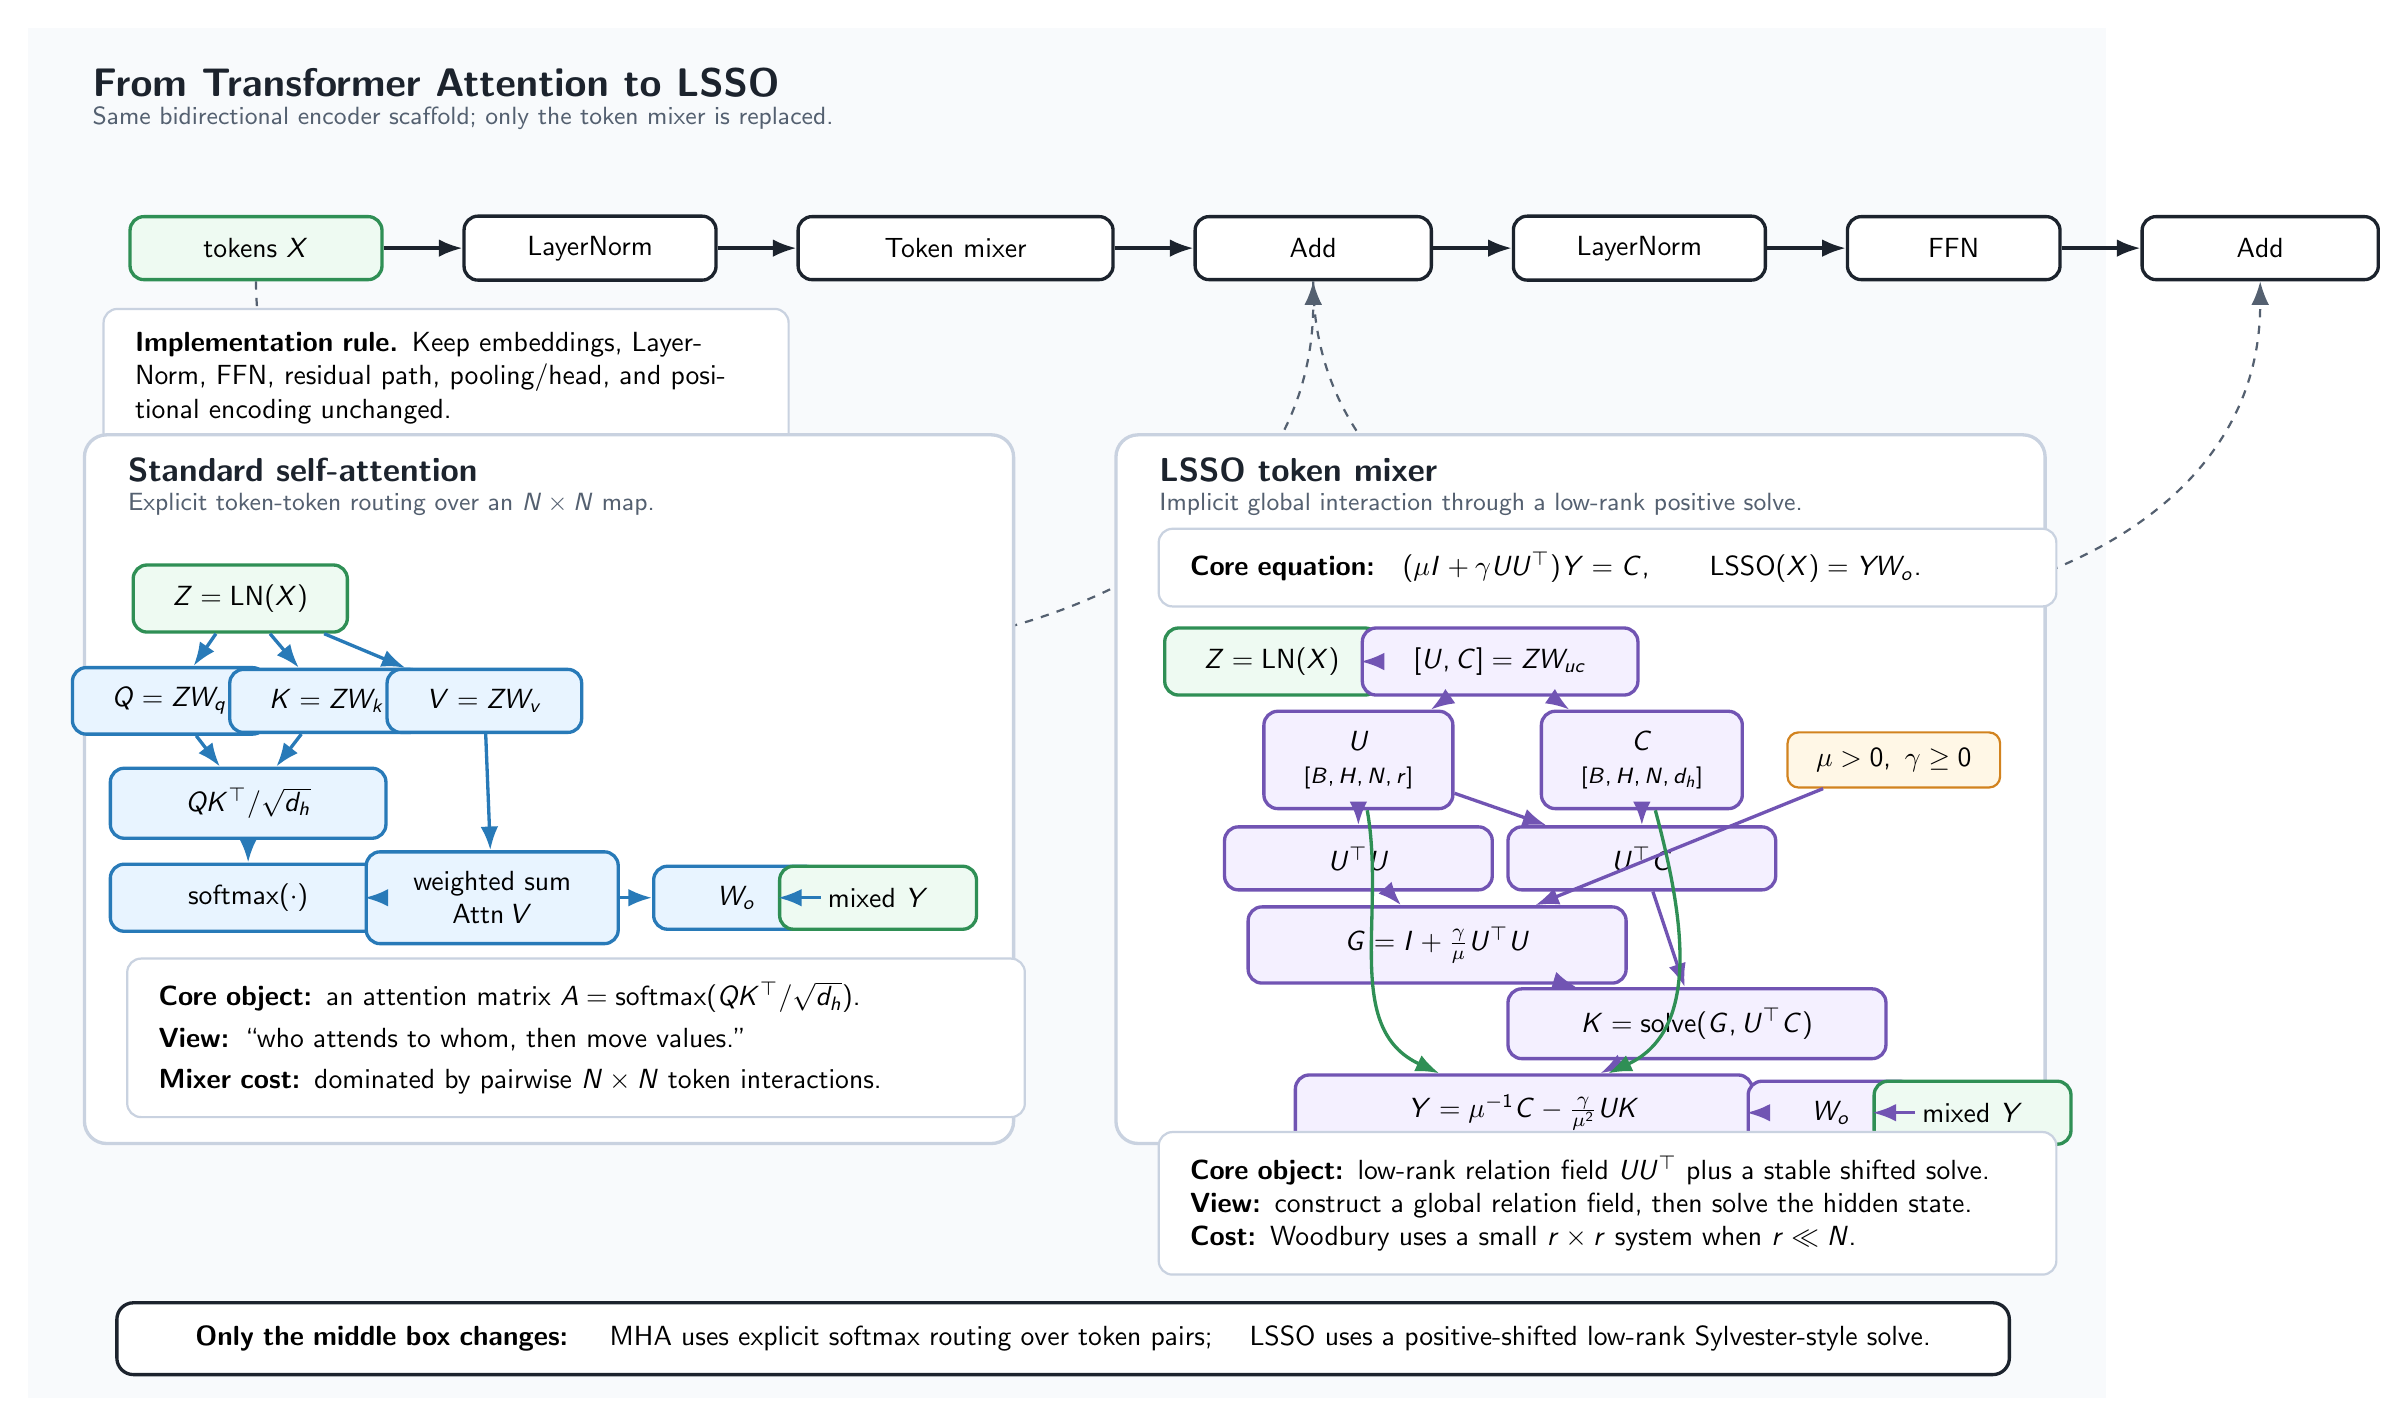
\begin{tikzpicture}[x=1cm,y=1cm]

% Background
\fill[paper] (-0.7,-2.0) rectangle (25.7,15.4);

% Title
\node[title, anchor=west] at (0,14.7) {From Transformer Attention to LSSO};
\node[subtitle, anchor=west] at (0,14.25)
  {Same bidirectional encoder scaffold; only the token mixer is replaced.};

% Shared scaffold
\node[stateBlock, minimum width=3.2cm] (x) at (2.2,12.6) {tokens $X$};
\node[block, minimum width=3.2cm, right=1.0cm of x] (ln1) {LayerNorm};
\node[block, minimum width=4.0cm, right=1.0cm of ln1] (mixer) {Token mixer};
\node[block, minimum width=3.0cm, right=1.0cm of mixer] (add1) {Add};
\node[block, minimum width=3.2cm, right=1.0cm of add1] (ln2) {LayerNorm};
\node[block, minimum width=2.7cm, right=1.0cm of ln2] (ffn) {FFN};
\node[block, minimum width=3.0cm, right=1.0cm of ffn] (add2) {Add};

\draw[arrow] (x) -- (ln1);
\draw[arrow] (ln1) -- (mixer);
\draw[arrow] (mixer) -- (add1);
\draw[arrow] (add1) -- (ln2);
\draw[arrow] (ln2) -- (ffn);
\draw[arrow] (ffn) -- (add2);
\draw[faintArrow] (x.south) to[out=-90,in=-90,looseness=1.2] node[caption, below] {residual} (add1.south);
\draw[faintArrow] (add1.south) to[out=-90,in=-90,looseness=1.2] node[caption, below] {residual} (add2.south);

\node[noteBlock, text width=7.9cm, anchor=west] at (0.25,10.95)
  {\textbf{Implementation rule.} Keep embeddings, LayerNorm, FFN, residual path, pooling/head, and positional encoding unchanged.};

% Panels
\node[panelBox, minimum width=11.8cm, minimum height=9.0cm, anchor=north west] (leftPanel) at (0,10.25) {};
\node[panelBox, minimum width=11.8cm, minimum height=9.0cm, anchor=north west] (rightPanel) at (13.1,10.25) {};

\node[title, font=\sffamily\bfseries\large, anchor=west] at (0.45,9.78)
  {Standard self-attention};
\node[subtitle, anchor=west] at (0.45,9.35)
  {Explicit token-token routing over an $N\times N$ map.};

\node[title, font=\sffamily\bfseries\large, anchor=west] at (13.55,9.78)
  {LSSO token mixer};
\node[subtitle, anchor=west] at (13.55,9.35)
  {Implicit global interaction through a low-rank positive solve.};

% Left: MHA
\node[stateBlock, minimum width=2.4cm] (mhaX) at (2.0,8.15) {$Z=\mathrm{LN}(X)$};
\node[mhaBlock, minimum width=1.8cm] (q) at (1.1,6.85) {$Q=ZW_q$};
\node[mhaBlock, minimum width=1.8cm] (k) at (3.1,6.85) {$K=ZW_k$};
\node[mhaBlock, minimum width=1.8cm] (v) at (5.1,6.85) {$V=ZW_v$};
\node[mhaBlock, minimum width=3.5cm] (score) at (2.1,5.55) {$QK^\top/\sqrt{d_h}$};
\node[mhaBlock, minimum width=3.5cm] (softmax) at (2.1,4.35) {$\mathrm{softmax}(\cdot)$};
\node[mhaBlock, minimum width=3.2cm] (route) at (5.2,4.35) {weighted sum\\$\mathrm{Attn}\,V$};
\node[mhaBlock, minimum width=2.1cm] (mhaWo) at (8.3,4.35) {$W_o$};
\node[stateBlock, minimum width=2.5cm] (mhaOut) at (10.1,4.35) {mixed $Y$};

\draw[mhaArrow] (mhaX) -- (q);
\draw[mhaArrow] (mhaX) -- (k);
\draw[mhaArrow] (mhaX) -- (v);
\draw[mhaArrow] (q) -- (score);
\draw[mhaArrow] (k) -- (score);
\draw[mhaArrow] (score) -- (softmax);
\draw[mhaArrow] (softmax) -- (route);
\draw[mhaArrow] (v) -- (route);
\draw[mhaArrow] (route) -- (mhaWo);
\draw[mhaArrow] (mhaWo) -- (mhaOut);

\node[noteBlock, text width=10.6cm, anchor=south west] at (0.55,1.55)
  {\textbf{Core object:} an attention matrix $A=\mathrm{softmax}(QK^\top/\sqrt{d_h})$.\\[1mm]
   \textbf{View:} ``who attends to whom, then move values.''\\[1mm]
   \textbf{Mixer cost:} dominated by pairwise $N\times N$ token interactions.};

% Right: LSSO
\node[noteBlock, text width=10.6cm, anchor=north west] at (13.65,9.05)
  {\textbf{Core equation:}\quad
   $(\mu I+\gamma UU^\top)Y=C,\qquad \mathrm{LSSO}(X)=YW_o.$};

\node[stateBlock, minimum width=2.4cm] (lssoX) at (15.1,7.35) {$Z=\mathrm{LN}(X)$};
\node[lssoBlock, minimum width=3.5cm] (wuc) at (18.0,7.35) {$[U,C]=ZW_{uc}$};
\node[lssoBlock, minimum width=2.4cm] (u) at (16.2,6.10) {$U$\\{\footnotesize $[B,H,N,r]$}};
\node[lssoBlock, minimum width=2.4cm] (c) at (19.8,6.10) {$C$\\{\footnotesize $[B,H,N,d_h]$}};
\node[smallblock, draw=amber, fill=amberfill, minimum width=2.7cm] (scale) at (23.0,6.10)
  {$\mu>0,\ \gamma\ge 0$};
\node[lssoBlock, minimum width=3.4cm] (utu) at (16.2,4.85) {$U^\top U$};
\node[lssoBlock, minimum width=3.4cm] (utc) at (19.8,4.85) {$U^\top C$};
\node[lssoBlock, minimum width=4.8cm] (g) at (17.2,3.75)
  {$G=I+\frac{\gamma}{\mu}U^\top U$};
\node[lssoBlock, minimum width=4.8cm] (solve) at (20.5,2.75)
  {$K=\mathrm{solve}(G,U^\top C)$};
\node[lssoBlock, minimum width=5.8cm] (wood) at (18.3,1.62)
  {$Y=\mu^{-1}C-\frac{\gamma}{\mu^2}UK$};
\node[lssoBlock, minimum width=2.1cm] (lssoWo) at (22.2,1.62) {$W_o$};
\node[stateBlock, minimum width=2.5cm] (lssoOut) at (24.0,1.62) {mixed $Y$};

\draw[lssoArrow] (lssoX) -- (wuc);
\draw[lssoArrow] (wuc) -- (u);
\draw[lssoArrow] (wuc) -- (c);
\draw[lssoArrow] (u) -- (utu);
\draw[lssoArrow] (u) -- (utc);
\draw[lssoArrow] (c) -- (utc);
\draw[lssoArrow] (scale) -- (g);
\draw[lssoArrow] (utu) -- (g);
\draw[lssoArrow] (g) -- (solve);
\draw[lssoArrow] (utc) -- (solve);
\draw[lssoArrow] (solve) -- (wood);
\draw[greenArrow] (u) to[out=-80,in=155] (wood);
\draw[greenArrow] (c) to[out=-75,in=25] (wood);
\draw[lssoArrow] (wood) -- (lssoWo);
\draw[lssoArrow] (lssoWo) -- (lssoOut);

\node[noteBlock, text width=10.6cm, anchor=south west] at (13.65,-0.45)
  {\textbf{Core object:} low-rank relation field $UU^\top$ plus a stable shifted solve.
   \quad \textbf{View:} construct a global relation field, then solve the hidden state.
   \quad \textbf{Cost:} Woodbury uses a small $r\times r$ system when $r\ll N$.};

% Difference strip
\node[draw=ink, very thick, rounded corners=6pt, fill=panel,
      text width=23.8cm, align=center, inner ysep=3mm] at (12.45,-1.25)
  {\textbf{Only the middle box changes:}
   \quad MHA uses explicit softmax routing over token pairs;
   \quad LSSO uses a positive-shifted low-rank Sylvester-style solve.};

\end{tikzpicture}
\end{document}
